% FILE: figures/vesicle_flickering.tex
% Vesicle flickering regime schematic

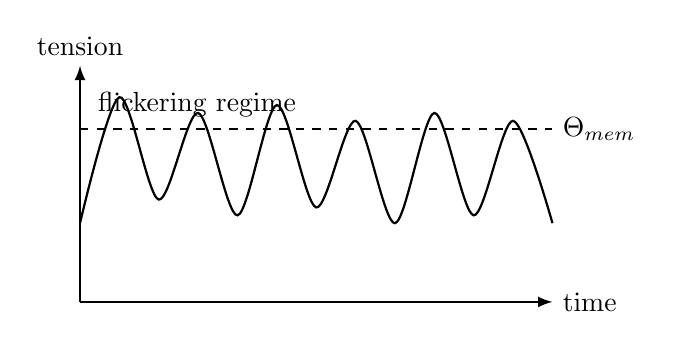
\begin{tikzpicture}[>=latex,thick,scale=1]
  % Time axis
  \draw[->] (0,0) -- (6,0) node[right] {time};
  \draw[->] (0,0) -- (0,3) node[above] {tension};

  % Threshold
  \draw[dashed] (0,2.2) -- (6,2.2);
  \node[anchor=west] at (6,2.2) {$\Theta_{\text{mem}}$};

  % Oscillatory tension
  \draw[smooth,thick]
    plot coordinates {
      (0.0,1.0)
      (0.5,2.6)
      (1.0,1.3)
      (1.5,2.4)
      (2.0,1.1)
      (2.5,2.5)
      (3.0,1.2)
      (3.5,2.3)
      (4.0,1.0)
      (4.5,2.4)
      (5.0,1.1)
      (5.5,2.3)
      (6.0,1.0)
    };

  \node[anchor=north west] at (0.1,2.8) {flickering regime};
\end{tikzpicture}
